\documentclass[sumlimits, intlimits]{beamer}

\usepackage[utf8]{inputenc}
\usepackage[T1]{fontenc}
\usepackage[english]{babel}
\usepackage{hyperref}
\usepackage{lmodern, microtype}
\usepackage[margin=2cm]{caption}
\usepackage{booktabs}
\usepackage{graphicx}

\usepackage{amsfonts, amsmath, amssymb}
\usepackage{mathtools}
\newcommand \twopi{{{\scriptstyle(2}\mskip-2.0mu\pi{\scriptstyle)}}}
\newcommand \ee{{\mathrm e}}
\newcommand \ii{{\mathrm i}}
\newcommand \full{{\mathrm d}}
\newcommand \fulld[1]{{\frac \full{\full {#1}}}}
\newcommand \partiald[1]{{\frac \partial{\partial {#1}}}}
\newcommand \yesnumber{\addtocounter{equation}{1}\tag \theequation}

\usepackage{listings}
\lstset{basicstyle=\footnotesize\ttfamily, tabsize=2}

\usepackage[backend=bibtex]{biblatex}
\addbibresource{refs.bib}

\title{ECMI Modelling Week 2018}
\subtitle{Storing Your Random Objects}
\author[shortname]{Desiré Nilsson \inst 1 \and
Ivana Gengeljacki \inst 5 \and
Jacob Hansen \inst 3 \and
Kirill Kiselev \inst 2 \and
Monika Žunji \inst 5 \and
Sampsa Kiiskinen \inst 4}
\institute[shortinst]{
\inst 1 Lund University \and
\inst 2 Saint Petersburg Polytechnic University \and
\inst 3 Technical University of Denmark \and
\inst 4 University of Jyväskylä \and
\inst 5 University of Novi Sad}
\date{2018-07-15 -- 2018-07-21}

\beamertemplatenavigationsymbolsempty

\usecolortheme{dove}
\usecolortheme{rose}
\usecolortheme{seahorse}

\mode<presentation>

\begin{document}

\begin{frame}
\titlepage
\end{frame}

\begin{frame}
\frametitle{Background}
\begin{block}{Problem Landscape}
\begin{itemize}
\item Packing spheres is well-established \cite{conway-1998},
but still not trivial \cite{torquato-2000}.
\item Packing more elaborate shapes has seen relatively little work,
because it is significantly more complicated.
\end{itemize}
\end{block}
\begin{block}{Challenges}
\begin{itemize}
\item Pen-and-paper analysis is limited to small systems.
\item Simulations provide little insight aside from the result.
\item Packing density is strongly protocol-dependent \cite{torquato-2002}.
\item Quantifying randomness
in a packing of spheres is tricky \cite{truskett-2000} and
in a packing of other shapes even trickier \cite{stoyan-1991}.
\end{itemize}
\end{block}
\end{frame}

\begin{frame}
\frametitle{Introduction}
\begin{block}{Problem Statement}
\begin{itemize}
\item Instead of trying to solve the most general problem,
we focused on a very specific instance.
\item What is the packing density and degree of randomness
in a collection of squares that is dropped into a square container?
\end{itemize}
\end{block}
\begin{block}{Relevance}
\begin{itemize}
\item Our problem should be directly applicable
to the prediction or optimization of industrial packaging processes.
\item Variations of our problem also appear
in the microstructural characterization
of heterogeneous materials \cite{torquato-2002}.
\end{itemize}
\end{block}
\end{frame}

\begin{frame}
\frametitle{Approaches}
\begin{block}{Bottom-to-Top Reconstruction}
\begin{itemize}
\item Use an event-driven simulation model
for the stacking of perfectly rigid objects \cite{poschel-2005}.
\item Fast, but may produce physically impossible results.
\item Had to be implemented from scratch.
\end{itemize}
\end{block}
\begin{block}{Discrete Element Method}
\begin{itemize}
\item Use a force-based simulation model
for the trajectories of elastic objects \cite{poschel-2005}.
\item Slow, but accurately represents reality when calibrated correctly.
\item Many existing implementations were available
(for example Box2D \cite{box2d} and Bullet \cite{bullet}).
\end{itemize}
\end{block}
\end{frame}

\begin{frame}
\frametitle{Restrictions}
\begin{block}{Protocol-Dependence}
The way the random arrangement is obtained has large impact on the resulting packing density for spheres \cite{torquato-2002},
so it is reasonable to believe that this is also true of squares.
Therefore the only option for obtaining realistic results is
to simulate the actual process.
\end{block}
\begin{block}{Friction and Elasticity}
Friction has a big effect on the outcome,
because larger friction is more prone to create configurations with higher potential energy.
Methods based on time integration have problems with inelastic particles,
because this makes the equations of motion stiff.
\end{block}
\end{frame}

\begin{frame}
\frametitle{Bottom-to-Top Reconstruction}
\begin{block}{Sketch of the Algorithm}
\centering
\def \h{7cm}
\only<1>{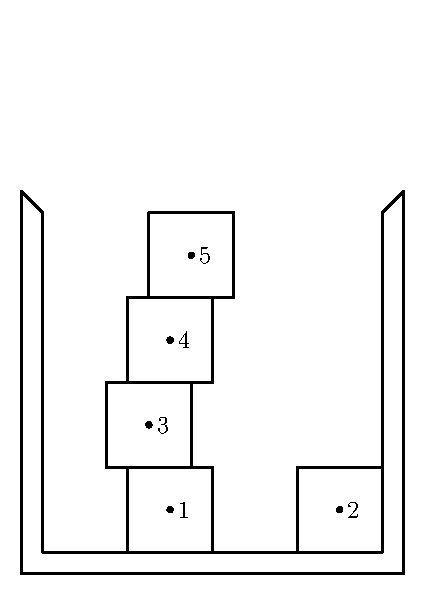
\includegraphics[height=\h]{btr-0}}%
\only<2>{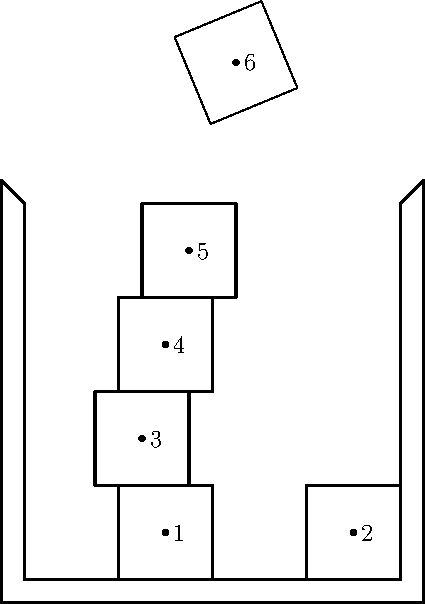
\includegraphics[height=\h]{btr-1}}%
\only<3>{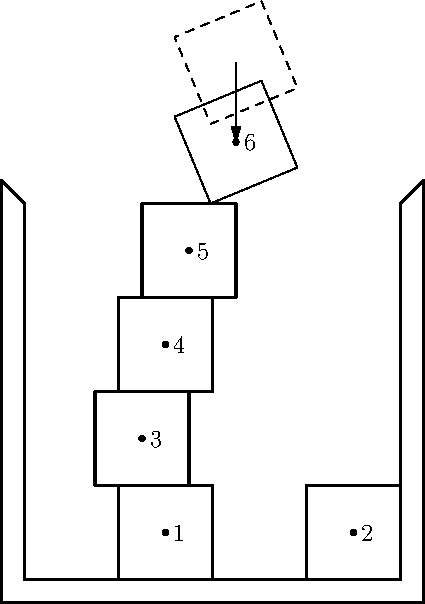
\includegraphics[height=\h]{btr-2}}%
\only<4>{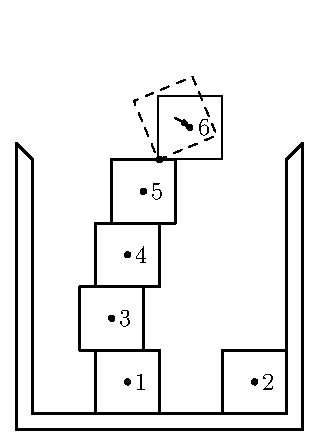
\includegraphics[height=\h]{btr-3}}%
\only<5>{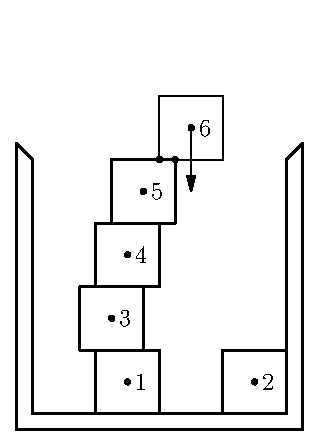
\includegraphics[height=\h]{btr-4}}%
\only<6>{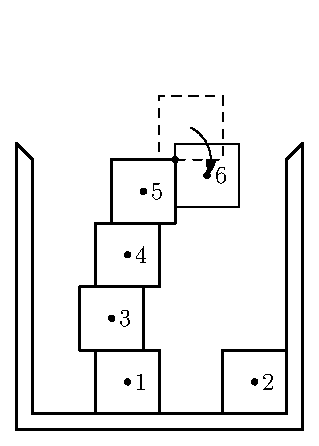
\includegraphics[height=\h]{btr-5}}%
\only<7>{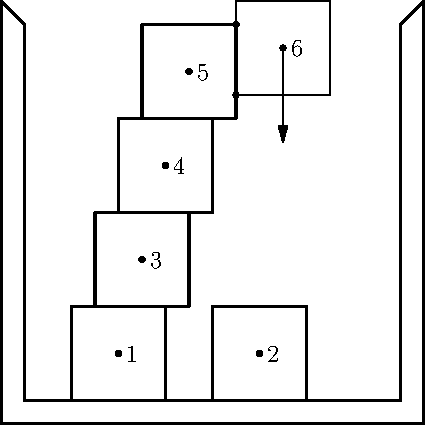
\includegraphics[height=\h]{btr-6}}%
\only<8>{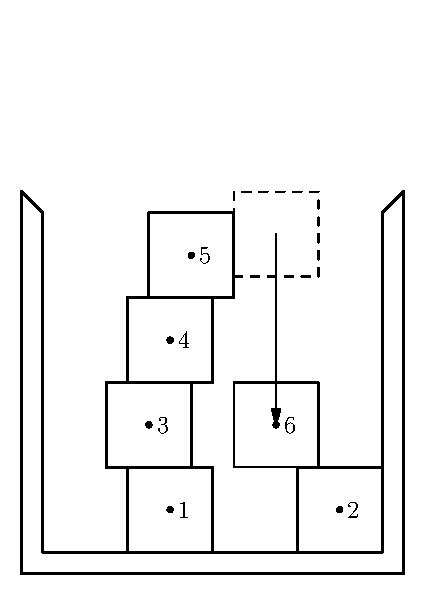
\includegraphics[height=\h]{btr-7}}%
\only<9>{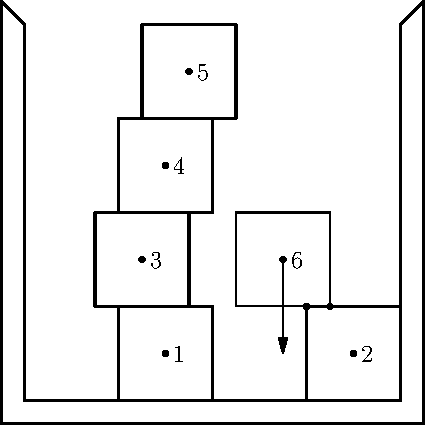
\includegraphics[height=\h]{btr-8}}%
\only<10>{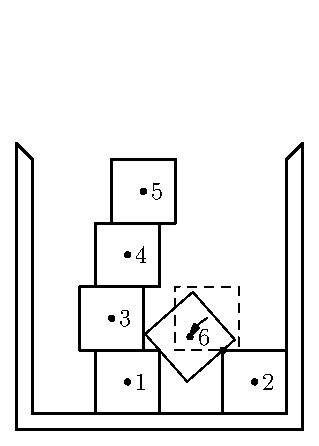
\includegraphics[height=\h]{btr-9}}%
\only<11>{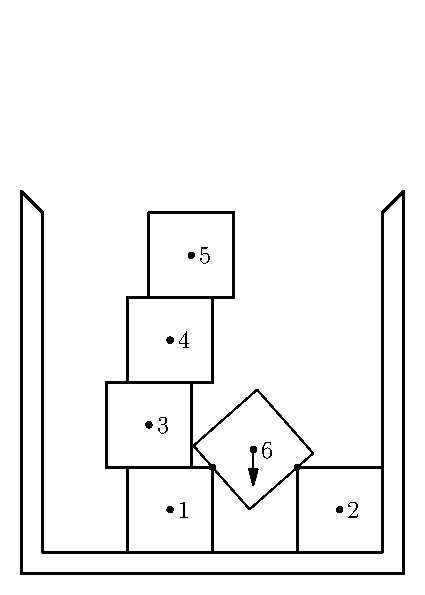
\includegraphics[height=\h]{btr-10}}%
\only<12>{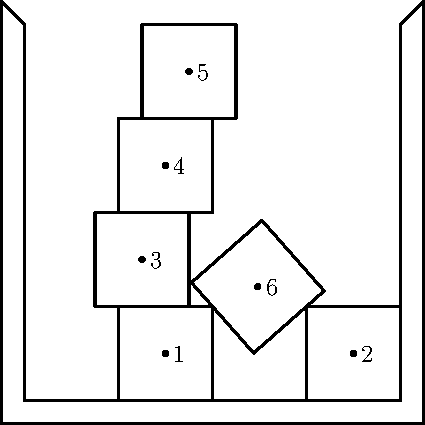
\includegraphics[height=\h]{btr-11}}
\end{block}
\end{frame}

\begin{frame}
\frametitle{Time Integration}
\begin{block}{Sketch of the Algorithm}
Figure goes here.
\end{block}
\end{frame}

\begin{frame}
\frametitle{Analysis}
\begin{block}{Packing Density}
We measured the packing density
\begin{align*}
\Delta & = \frac 1 V \sum_{i = 1}^N v_i,
\end{align*}
where $V$ is the volume of the container,
$N$ is the number of objects and
$v_i$ is the volume of the object $i$.
\end{block}
\end{frame}

\begin{frame}
\frametitle{Analysis}
\begin{block}{Randomness}
We also attempted to measure randomness.
Since the objects were not spherical,
it was difficult to find a suitable order metric.
We settled with the orientational correlation function
\begin{align*}
g & = \frac{\sum_{i = 1}^N \sum_{j = i + 1}^N (|\vec x_j - \vec x_i| < r) \max_{k, l} \cos 4 \arccos (\vec n_{i, k} \cdot \vec n_{j, l})}
{\sum_{i = 1}^N \sum_{j = i + 1}^N (|\vec x_j - \vec x_i| < r)},
\end{align*}
where $r$ is the nearest-neighbor range and
$\vec n_{i, k}$ is the $k$th surface normal of the object $i$.
The magic number $4$ comes from the size of the rotational symmetry group of the square.
\end{block}
\end{frame}

\begin{frame}
\frametitle{References}
\printbibliography
\end{frame}

\end{document}
